\documentclass[12pt, Tahoma]{article}

%%%%%%%%%%%%%%%%%%%%%%%%%%%%%%%%%%%%%%%%%%%%%%%%%%%%%%%%%%%%%%%%%%%%%%%%%%%%%%%%%%%

\usepackage{amsmath, amssymb, latexsym}
\usepackage{graphicx}
\usepackage{listings}
\usepackage{xcolor}
\usepackage{enumerate}
\usepackage{enumitem}
\usepackage{float}
\usepackage{subcaption}
\usepackage{setspace}
\usepackage{dirtytalk}

%%%%%%%%%%%%%%%%%%%%%%%%%%%%%%%%%%%%%%%%%%%%%%%%%%%%%%%%%%%%%%%%%%%%%%%%%%%%%%%%%%%

\begin{document}
	\title{
		Instituto Politecnico Nacional\\
		Escuela Superior de Cómputo\\
		Desarrollo de aplicaciones para analisis de datos\\
		\vspace{1cm}
			\textbf{Proyecto - Parte 3}\\
			\textbf{En busca de una estrategia ganadora para el juego \say{El ratón y los gatos} en un tablero de Ajedrez (Pt 3)}
	}
	\author{
		Valdés Nava Javier\\
		Trujano Ortíz Luís Antonio\\
		Ivan Uriel Rosario Margarito
	}
	\date{30 de Junio del 2025}
	\maketitle
	\section*{Objetivo:} Definido el experimento \say{Jugar una partida de Ratón y los gatos como el jugador que controla al Ratón}, y dado un cierto estado del juego, buscar cual es la mejor decisión a tomar acorde a ese estado, hasta que se encuentre la serie de decisiones que para ese estado en especifico resulten en una victoria. Siendo esa serie de decisiones una \say{Estrategia ganadora}. El experimento se repetirá hasta que aquel que lo realiza considere que ya es correcto detenerse o hasta que encontremos todas las posibles estrategias ganadoras.
	\section*{Justificacion} El proyecto fue inspirado en los distintos libros de estrategias de ajedrez que existe.
	 
	 
	Dado que el juego del Raton y los Gatos tiene muchas similitudes con el ajedrez, creemos que es posible encontrar al menos una estrategia para el jugador que maneja el ratón. Para lograr una victoria bajo un cierto estado del juego.
	
	
	Deseamos recabar datos de las partidas como los movimientos que realiza un jugador Raton, los movimientos que realiza un jugador Gato y el resultado de la partida, en esperanza de encontrar un patrón de movimientos que siempre determinan el resultado de un juego.
	
	
	Esta información puede ser útil para jugadores competitivos que quieran mejorar su estilo de juego para lograr o evitar llegar a los estados que obliguen a finalizar el juego. O a los jueces y arbitros del juego para determinar la probabilidad de victoria de cierto jugador en caso de que el juego tuviera que parar por circunstancias externas y no se llegara a un resultado (Problema del Caballo de Méré de Pascal y Fermat para apuestas interrumpidas).
	 
	\section*{Diagrama de Clases}
	\begin{figure}[H]
		\centering
		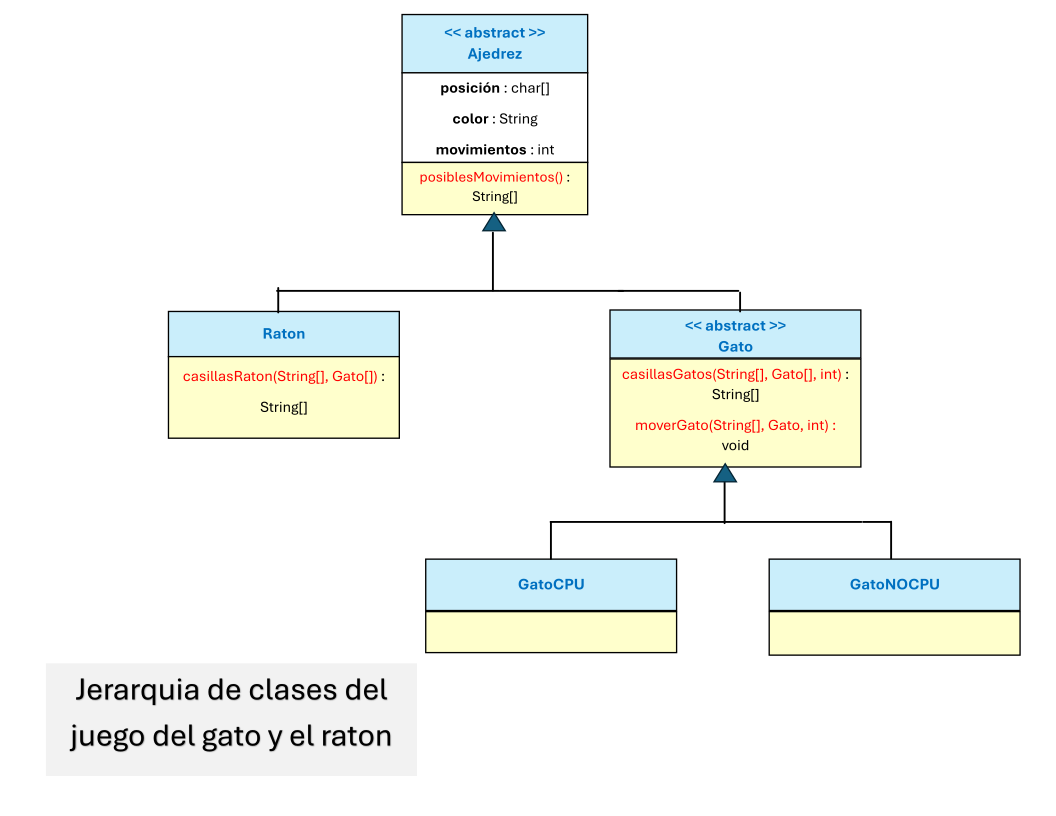
\includegraphics[scale=0.6]{gatoRaton.png}
	\end{figure}
	\section*{Implementacion en Python}
	\begin{figure}[H]
		\centering
		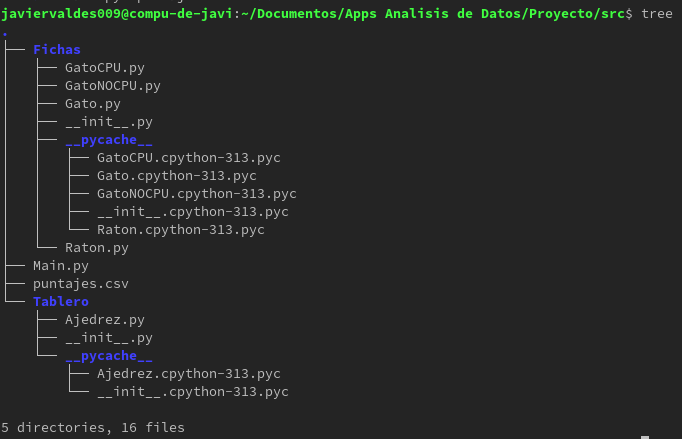
\includegraphics[scale=0.6]{Paquetes2.png}
	\end{figure}
	\begin{figure}[H]
		\centering
		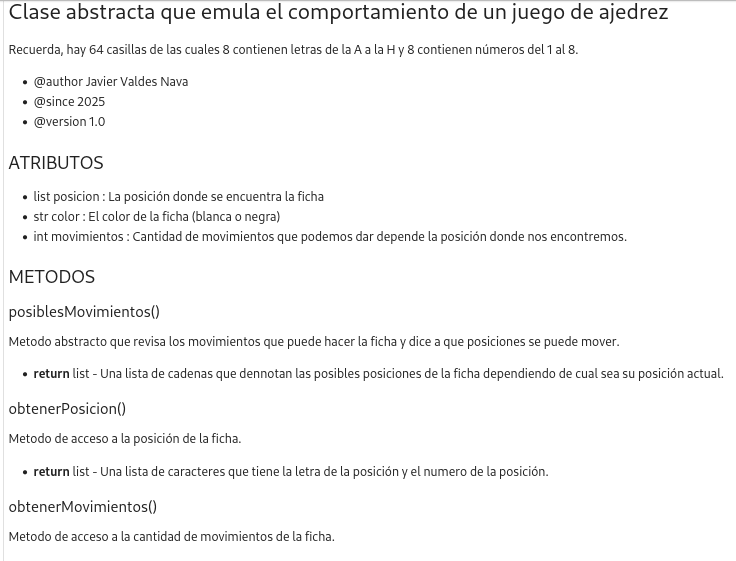
\includegraphics[scale=0.6]{ClaseAjedrez1.png}
	\end{figure}
	\begin{figure}[H]
		\centering
		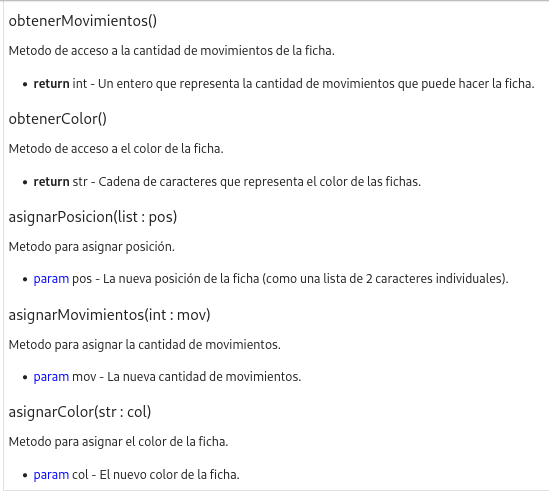
\includegraphics[scale=0.6]{ClaseAjedrez2.png}
	\end{figure}
	\begin{figure}[H]
		\centering
		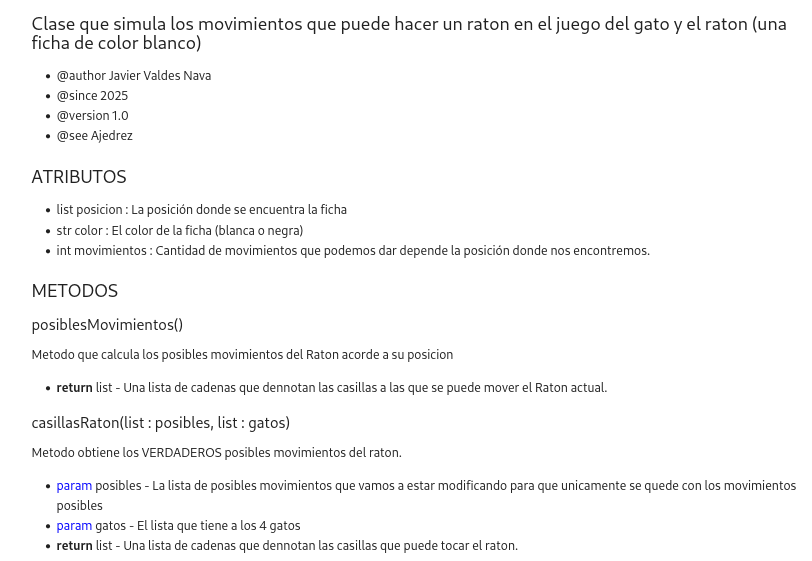
\includegraphics[scale=0.6]{ClaseRaton.png}
	\end{figure}
	\begin{figure}[H]
		\centering
		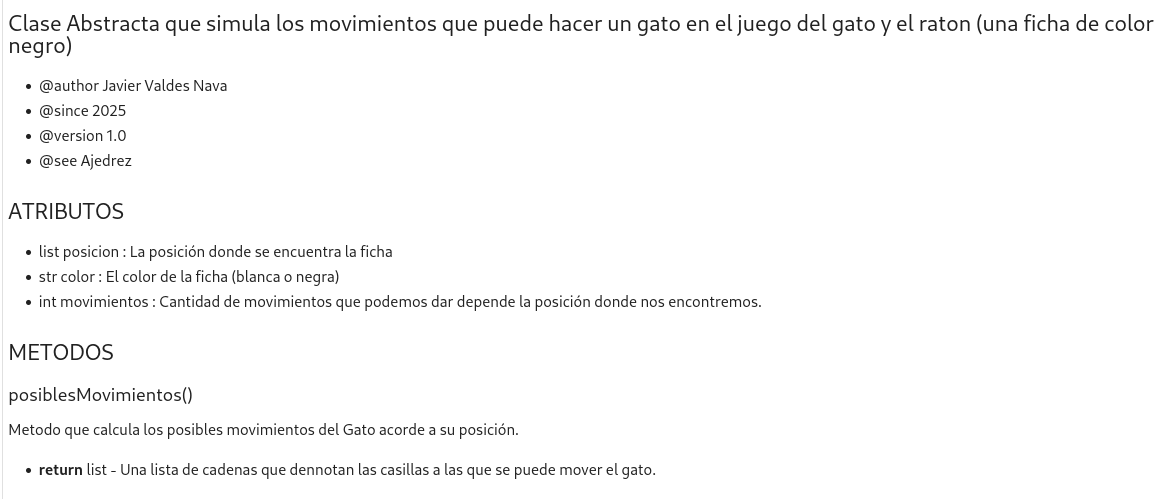
\includegraphics[scale=0.4]{ClaseGato1.png}
	\end{figure}
	\begin{figure}[H]
		\centering
		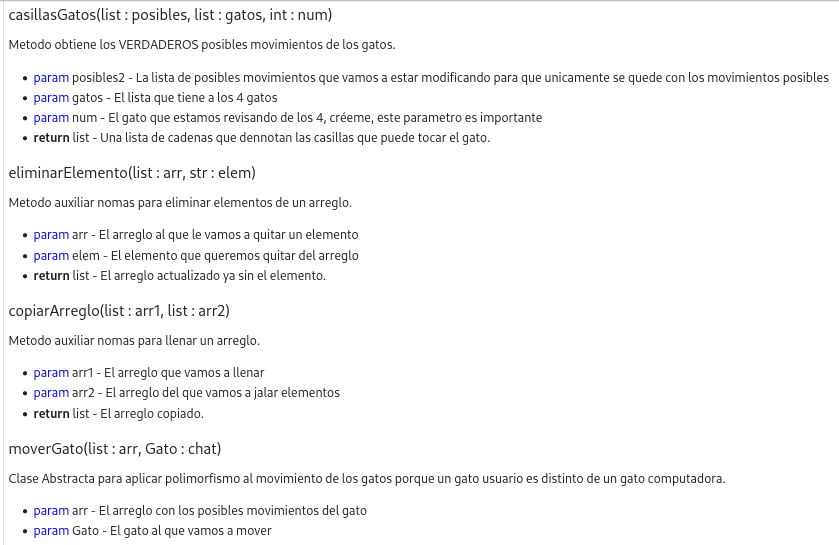
\includegraphics[scale=0.5]{ClaseGato2.png}
	\end{figure}
	\begin{figure}[H]
		\centering
		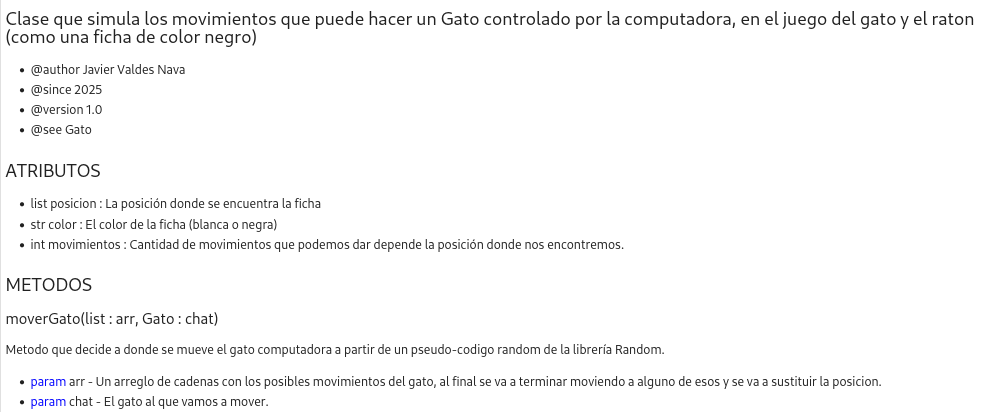
\includegraphics[scale=0.5]{ClaseGatoCPU.png}
	\end{figure}
	\begin{figure}[H]
		\centering
		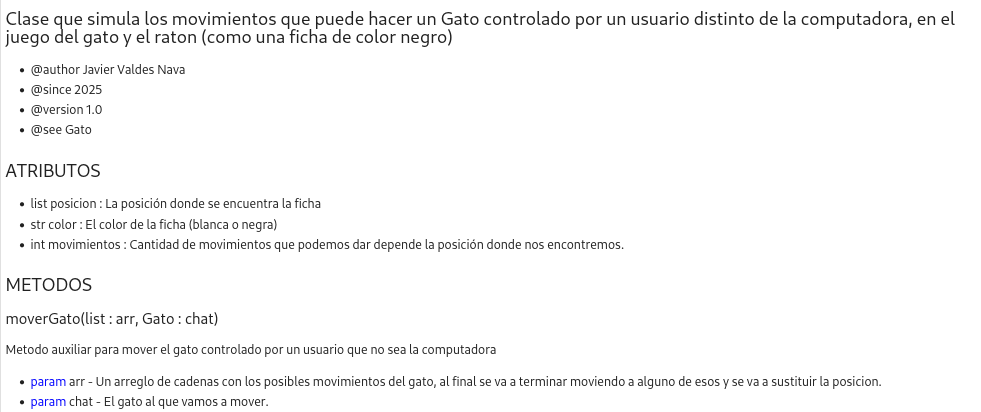
\includegraphics[scale=0.5]{ClaseGatoNOCPU.png}
	\end{figure}
	
	
	\section*{Instrucciones de cómo correr esta implementación}
	
	
	Lo primero es instalar Python3 (cualquier version, preferiblemente la mas reciente). En windows puedes instalarla mediante el siguiente enlace\\ \textbf{\textcolor{cyan}{\underline{https://www.python.org/downloads/}}}
	
	
	Una vez instalado python, instala las siguientes librerias de Python:
	
	
	Libreria $|$ Comando (en terminal o linea de comandos)
	\begin{itemize}
		\item Numpy : \$ pip install numpy
		\item MatPlotLib : \$ pip install matplotlib
		\item Pandas : \$ pip install pandas
		\item Plotly : \$ pip install plotly
	\end{itemize}
	
	
	Si se utiliza Google Colab, no es necesario instalar las otras librerias, ya vienen preinstaladas (excepto plotly, para eso, utilizas \%pip install plotly).
	
	
	Para correr esta implementación en terminal puedes seguir los siguientes pasos:
	\begin{enumerate}
		\item Accede al repositorio con el enlace web: \\ 
		\textbf{\textcolor{cyan}{\underline{https://github.com/JavierVN009/Proyecto\_DAAD.git}}}
		\item Da click en el botón verde con la leyenda "Code" 
			\begin{figure}[H]
				\centering
				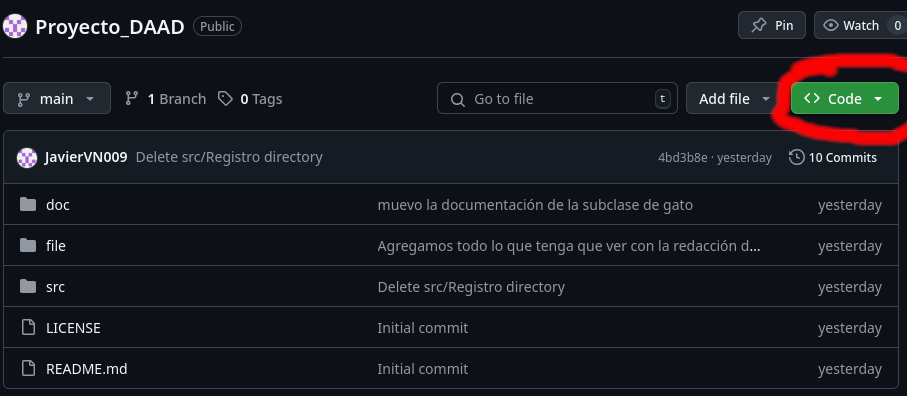
\includegraphics[scale= 2]{correr1.png}
			\end{figure}
		\item  Se despliega un menú, al final del menú se puede leer "Download ZIP", dar click en "Download ZIP", se comenzará a descargar el comprimido. 
			\begin{figure}[H]
				\centering
				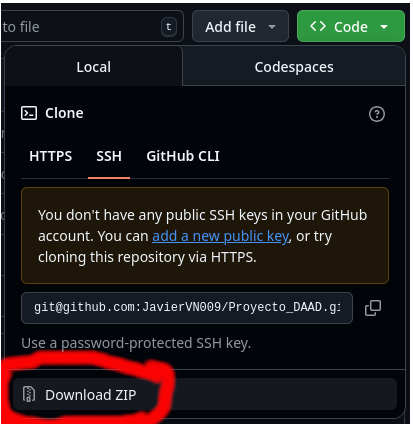
\includegraphics[scale=2]{correr2.png}
			\end{figure}
		\item  Una vez que se descargo el archivo, dirígete a la ubicación donde está el archivo comprimido (muy probablemente en descargas) y descomprimelo. \\ Si utilizas WinRAR, al descomprimir obtendrás 3 directorios
		\begin{itemize}
			\item src
			\item file
			\item doc
		\end{itemize}
		En caso contrario, obtendras un directorio llamado \say{Proyecto DAAD} con los mismos tres directorios en su interior.
		\item Abre el directorio "src".
			\begin{figure}[H]
				\centering
				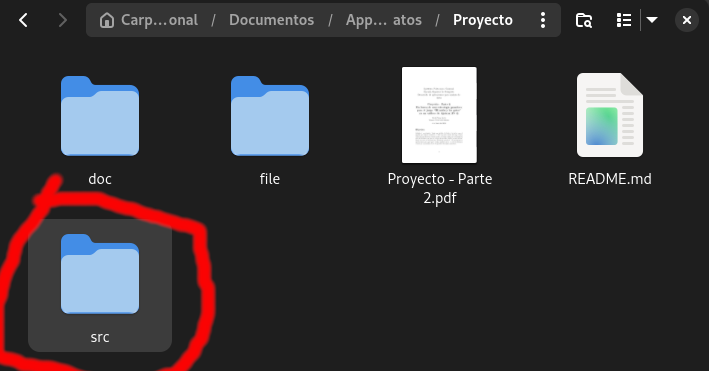
\includegraphics[scale=2]{correr4.png}
			\end{figure}
		\item Copia la dirección del directorio src 
			\begin{figure}[H]
				\centering
				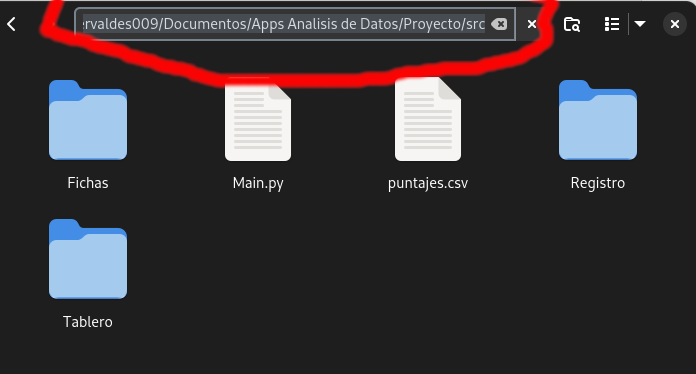
\includegraphics[scale=2]{correr3.png}
			\end{figure}
		\item Abre la terminal/cmd de tu equipo 
			\begin{figure}[H]
				\centering
				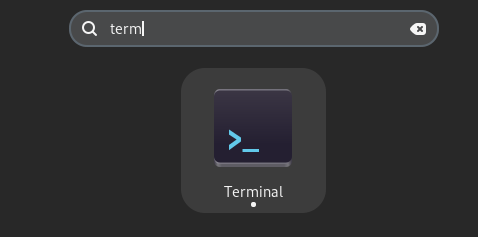
\includegraphics[scale=2]{correr5.png}
			\end{figure}
		\item Teclea "cd " y después, pega la dirección que copiaste y presiona ENTER.
			\begin{figure}[H]
				\centering
				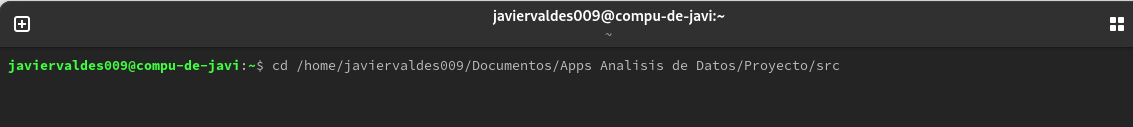
\includegraphics[scale=0.4]{correr6.png}
			\end{figure}
		\item Teclea "python3 Main.py"
			\begin{figure}[H]
				\centering
				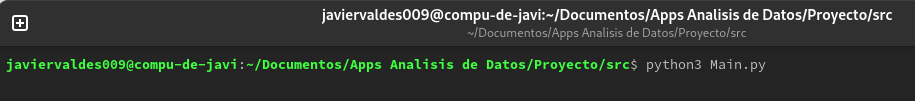
\includegraphics[scale=0.5]{correr7.png}
			\end{figure}
		 \item  Sigue las instrucciones dentro del programa.
		 	\begin{figure}[H]
				\centering
				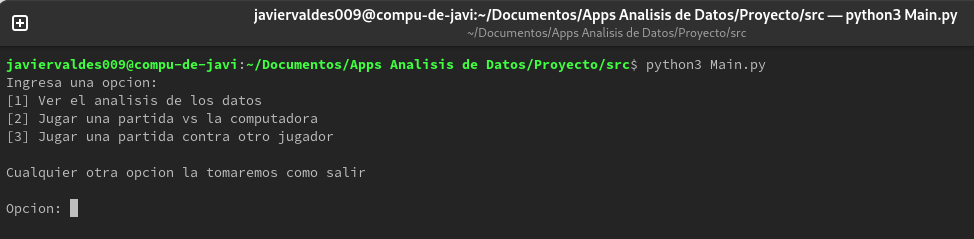
\includegraphics[scale=0.5]{correr8.png}
			\end{figure}
	\end{enumerate}
	
	
	NOTA, también puedes clonar el repositorio usando: 
	\begin{center}
		\textcolor{green}{\$} \textcolor{gray}{\textbf{git clone \say{enlace}}} 
	\end{center}
	
	Para correr el programa en Google Colab es un poco más complicado, pero puede seguirse el siguiente procedimiento
	\begin{enumerate}
		\item Abrimos google Colab.
		\item Creamos un nuevo notebook y lo llamamos \say{Main}
			\begin{figure}[H]
				\centering
				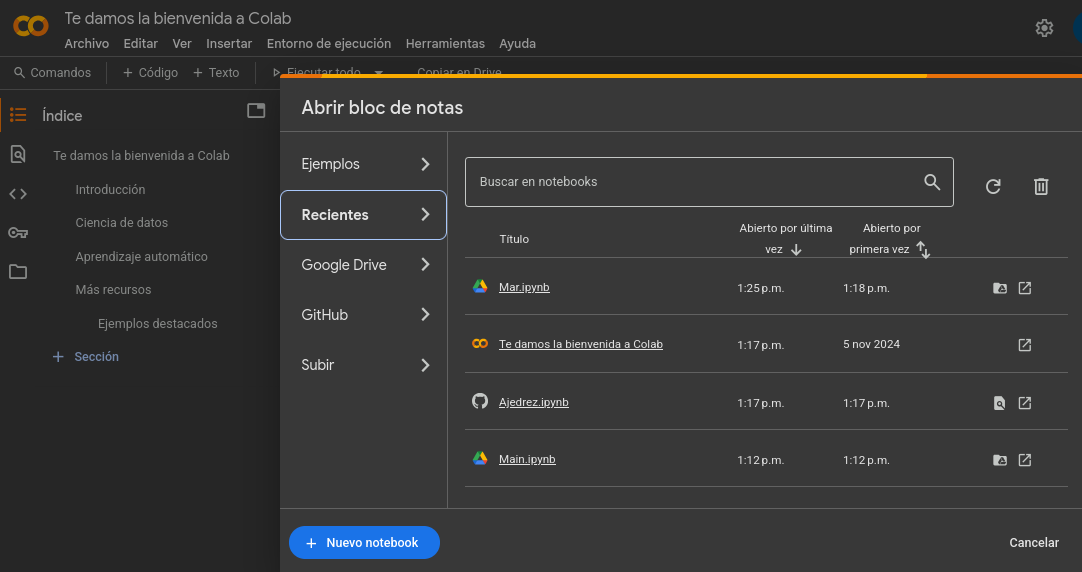
\includegraphics[scale=0.3]{correr9.png}
			\end{figure}
			\begin{figure}[H]
				\centering
				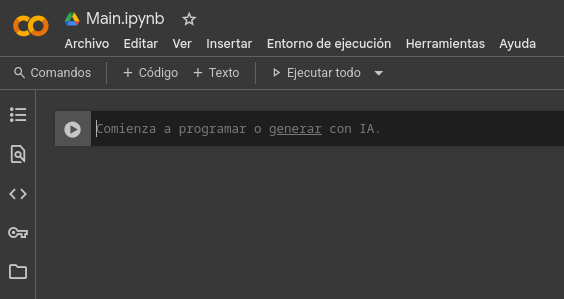
\includegraphics[scale=0.6]{correr10.png}
			\end{figure}
		\item Abrimos la sección de \say{Archivos}
			\begin{figure}[H]
				\centering
				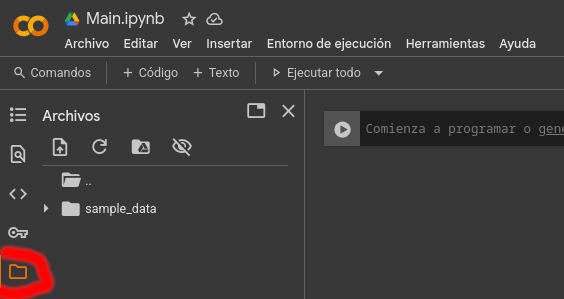
\includegraphics[scale=2]{correr11.png}
			\end{figure}
		\item Damos click en el icono de una hoja doblada por el borde derecho y con una flecha apuntando hacia arriba (\say{Cargar archivos al almacenamiento de sesión}).
		\item Nos dirigimos a la carpeta \say{src} de nuestro proyecto
			\begin{figure}[H]
				\centering
				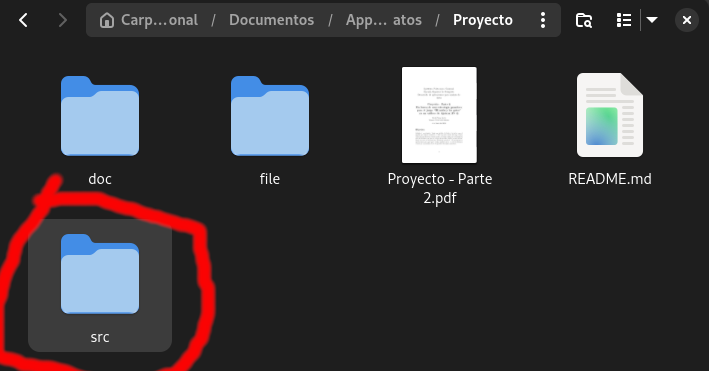
\includegraphics[scale=1.5]{correr4.png}
			\end{figure}
		\item Abrimos el directorio \say{Tablero}
			\begin{figure}[H]
				\centering
				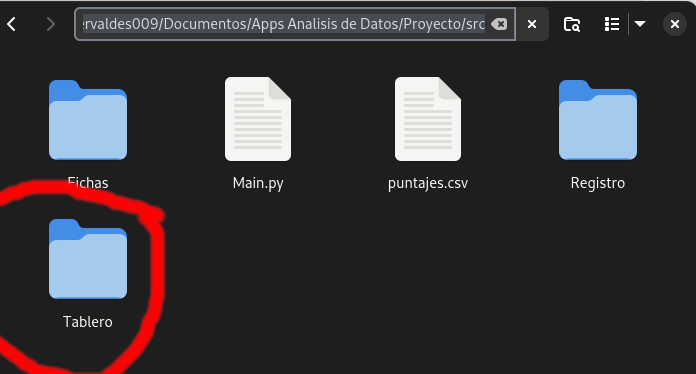
\includegraphics[scale=1.5]{correr12.png}
			\end{figure}
		\item Seleccionamos el archivo \say{Ajedrez.py} y lo cargamos (dando Enter en el teclado).
			\begin{figure}[H]
				\centering
				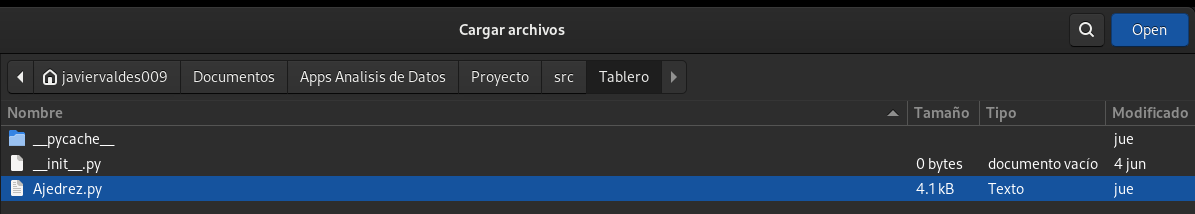
\includegraphics[scale=1.5]{correr13.png}
			\end{figure}
		\item Hacemos lo mismo para el directorio \say{Fichas} con los archivos \say{Gato.py}, \say{GatoCPU.py}, \say{GatoNOCPU.py} y \say{Raton.py}
			\begin{figure}[H]
				\centering
				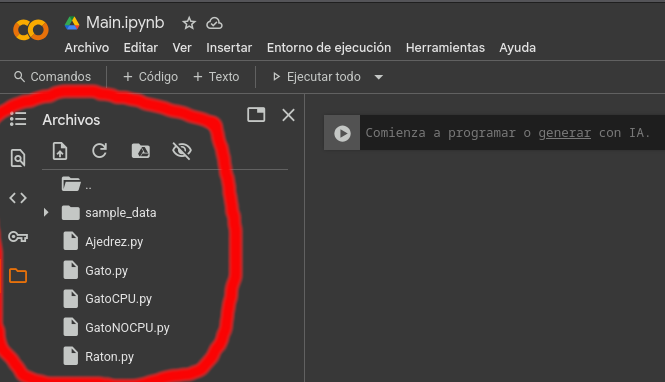
\includegraphics[scale=2]{correr14.png}
			\end{figure}
		\item Ya que tenemos todos los archivos cargados en Colab, Damos click derecho en alguna sección libre (por ejemplo, la sección debajo del archivo \say{Raton.py}), se desplegará un pequeño menú, seleccionamos la opcion que dice \say{Nueva carpeta} y damos click izquierdo.
			\begin{figure}[H]
				\centering
				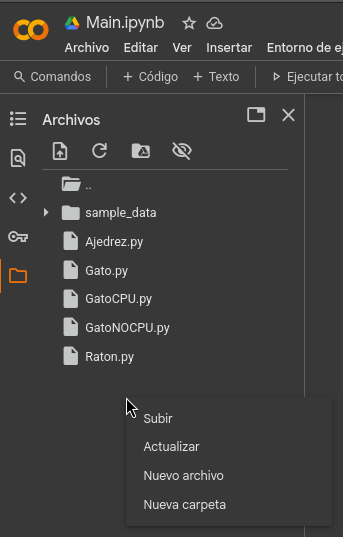
\includegraphics[scale=0.6]{correr15.png}
			\end{figure}
		\item A la nueva carpeta la llamamos \say{Tablero}
			\begin{figure}[H]
				\centering
				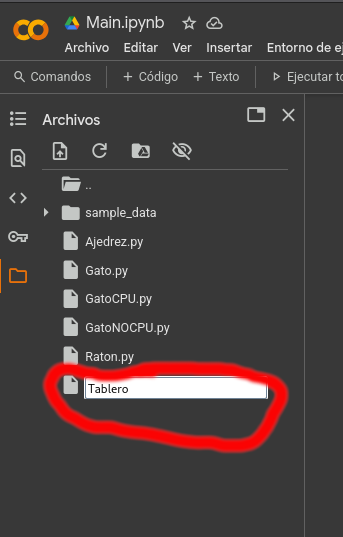
\includegraphics[scale=2]{correr16.png}
			\end{figure}
		\item Mantenemos click izquierdo sobre el archivo \say{Ajedrez.py} y lo arrastramos hacia la carpeta \say{Tablero}
			\begin{figure}[H]
				\centering
				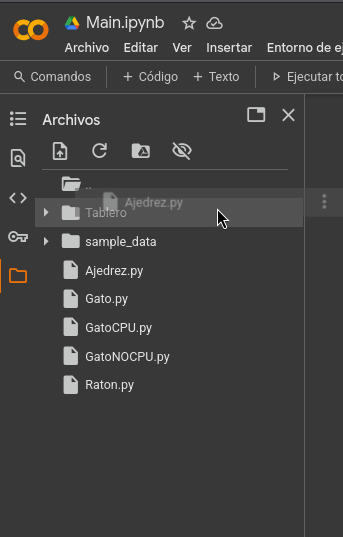
\includegraphics[scale=0.6]{correr17.png}
			\end{figure}
		\item Creamos una carpeta llamada \say{Fichas} y arrastramos a ella c/u de los archivos restantes (es decir, \say{Gato.py}, \say{GatoCPU.py}, \say{GatoNOCPU.py} y \say{Raton.py})
			\begin{figure}[H]
				\centering
				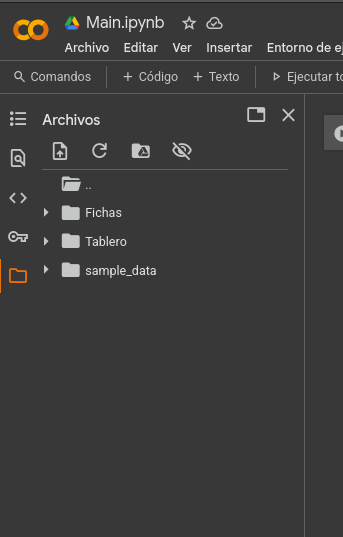
\includegraphics[scale=2]{correr18.png}
			\end{figure}
		\item Ya que tenemos todo en orden, simplemente abrimos nuestro archivo \say{Main.py} que está dentro del directorio \say{src}, copiamos su contenido, y lo pegamos en Colab.
			\begin{figure}[H]
				\centering
				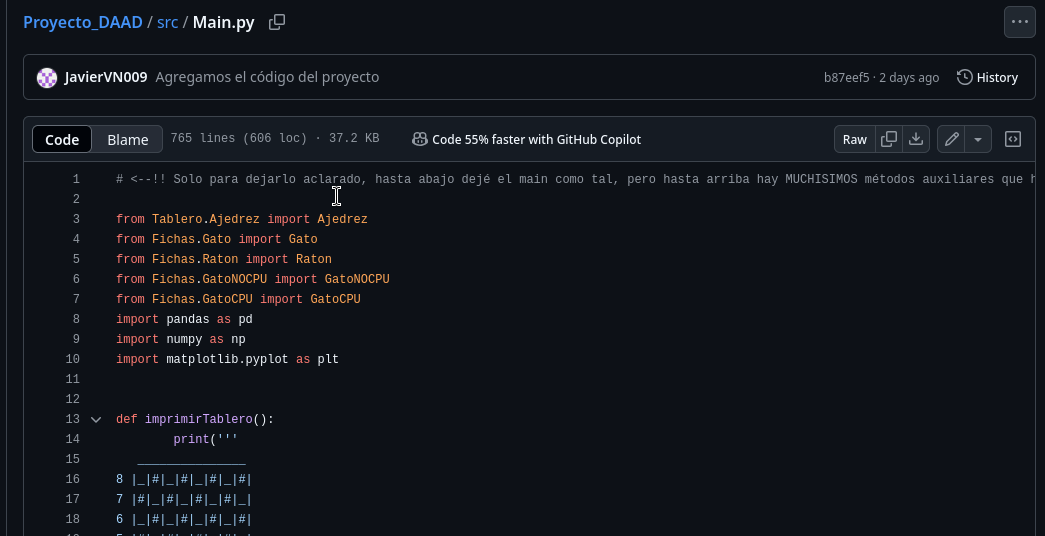
\includegraphics[scale=0.4]{correr19.png}
			\end{figure}
			\begin{figure}[H]
				\centering
				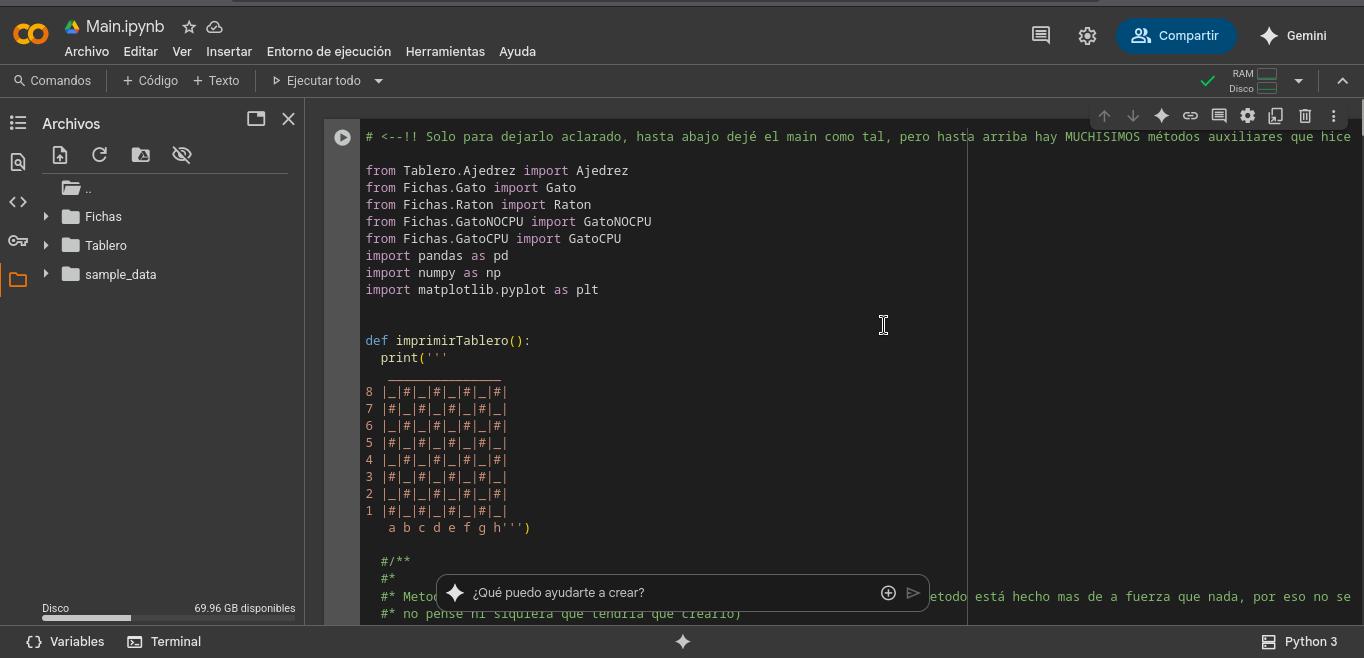
\includegraphics[scale=0.3]{correr20.png}
			\end{figure}
		\item Simplemente lo corremos y seguimos las instrucciones dentro del programa.
			\begin{figure}[H]
				\centering
				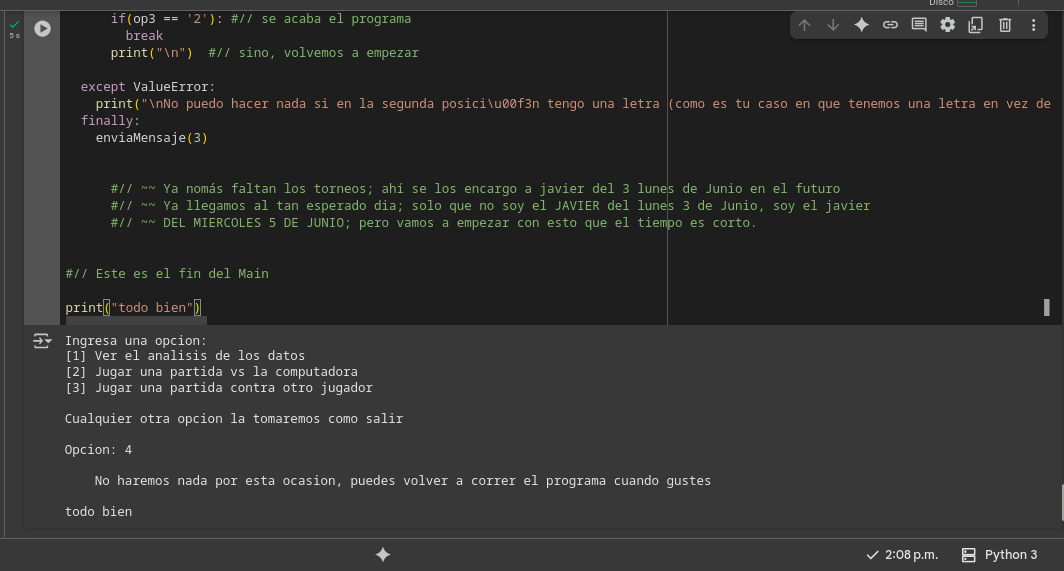
\includegraphics[scale=0.4]{correr21.png}
			\end{figure}
	\end{enumerate}
	
	
	NOTA: Puedes simplemente abrir desde el Colab, el archivo \say{Main.ipynb} en vez de copiar y pegar todo el código del Main.
	
	
	Para correr el código en Jupyter Notebook es muchisimo más fácil, simplemente sigue estos pasos:
	\begin{enumerate}
		\item Copia la dirección del directorio src 
			\begin{figure}[H]
				\centering
				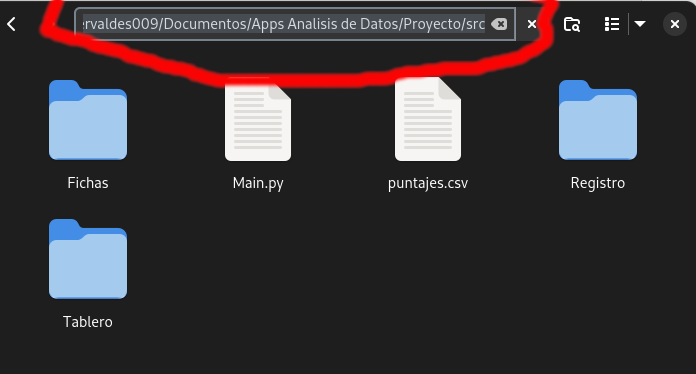
\includegraphics[scale=2]{correr3.png}
			\end{figure}
		\item Abre la terminal y teclea "cd " y después, pega la dirección que copiaste y presiona ENTER.
			\begin{figure}[H]
				\centering
				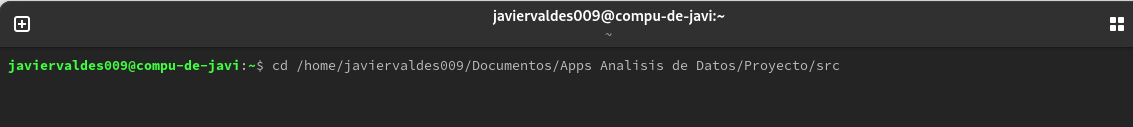
\includegraphics[scale=0.4]{correr6.png}
			\end{figure}
		\item Teclea \say{jupyter notebook}
			\begin{figure}[H]
				\centering
				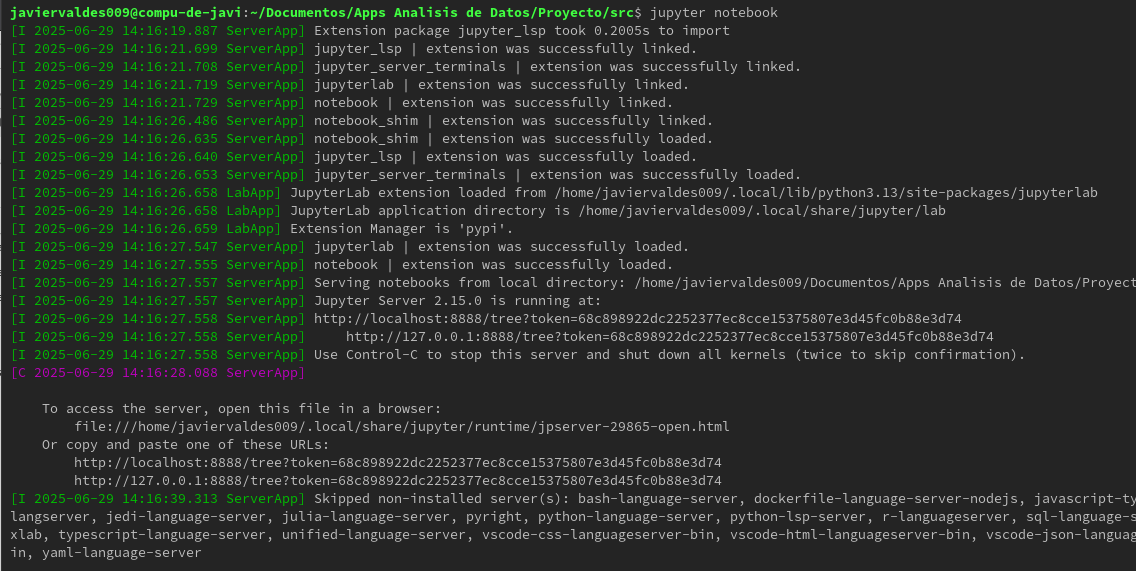
\includegraphics[scale=0.3]{correr22.png}
			\end{figure}
		\item Abre el archivo \say{Main.ipynb}
			\begin{figure}[H]
				\centering
				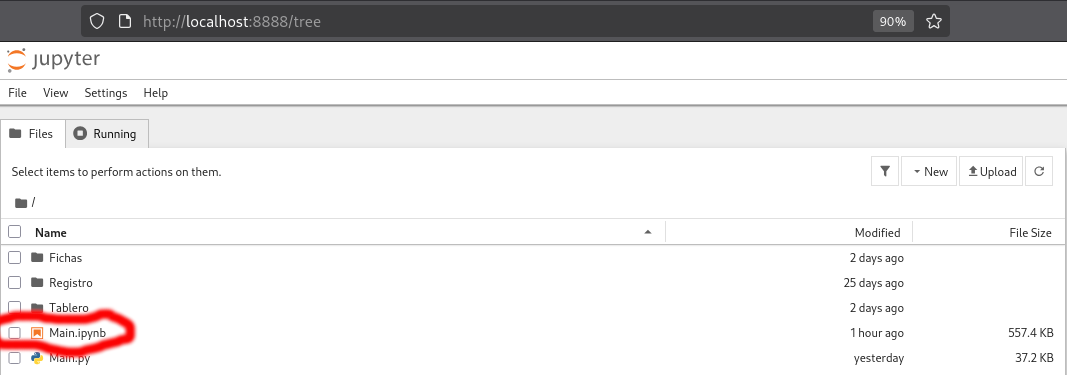
\includegraphics[scale=1.6]{correr23.png}
			\end{figure}
		\item Corre la celda y sigue las instrucciones del programa.
	\end{enumerate}
	
	
	Elige la opción que más te guste, ya sabes como correr todas :D.
	
	\section*{Resumen del funcionamiento de la aplicación y resultados obtenidos con ella}
	La aplicación tiene 2 usos principales; uno como un PyGame que puedes jugar solo o con la computadora, y del cual recabamos todos los datos que analizamos para el proyecto (pues es precisamente el juego del gato y el ratón). Y el segundo como un analizador de movimientos el cual simplemente agrupa todos los movimientos (como conjunto sin repeticiones), cuenta las veces que se gana con esos movimientos, cuantas veces se pierde, obtiene las probabilidades de todo el historico de juegos de ganar con esos movimientos (utilizando el enfoque de probabilidad frecuentista) y nos muestra una tablita con la información por movimientos (similar a las famosas tablas de probabilidades de aparición de Manos de Poker), y un gráfico de barras que sirven para visualizar mejor como ciertos movimientos tienen mayor probabilidad de dar una victoria contra otros (e incluso poder determinar una distribución para la probabilidad de los movimientos).
	
	
	El análisis es simple, guardamos en un registro (como un DataFrame):
	\begin{itemize}
		\item Una columna que sea “Las casillas por las que se movió el ratón” 
		\item Una columna que sea “La cantidad de turnos que se jugaron antes de acabar el juego”
		\item Una columna que sea “El resultado del juego (ganó o perdió el ratón)” 
	\end{itemize}

	Una vez que lo tenemos como DataFrame, agrupamos por la primera columna, contamos el total de veces que ganó con esa exacta serie de movimientos, calculamos la probabilidad con el enfoque frecuentista (con historico de juegos que se han jugado como espacio muestral) y le agregamos la proba de ganar como columna a el agrupado.


	Al finalizar el analisis, se hicieron dos gráficos de Barras para c/u de los grupos. Uno con las probabilidades de ganar, y otro con las probabilidades de perder (para hacer comparaciones) 


	La información del CSV la guardamos al final de cada partida jugada (y si no existe el CSV, lo crea, es un simple manejo de un Try-Except).  
	
	
	Estos son los resultados que se obtienen de ella: \\
	\textbf{Uso como analizador: }
	\begin{figure}[H]
		\centering
		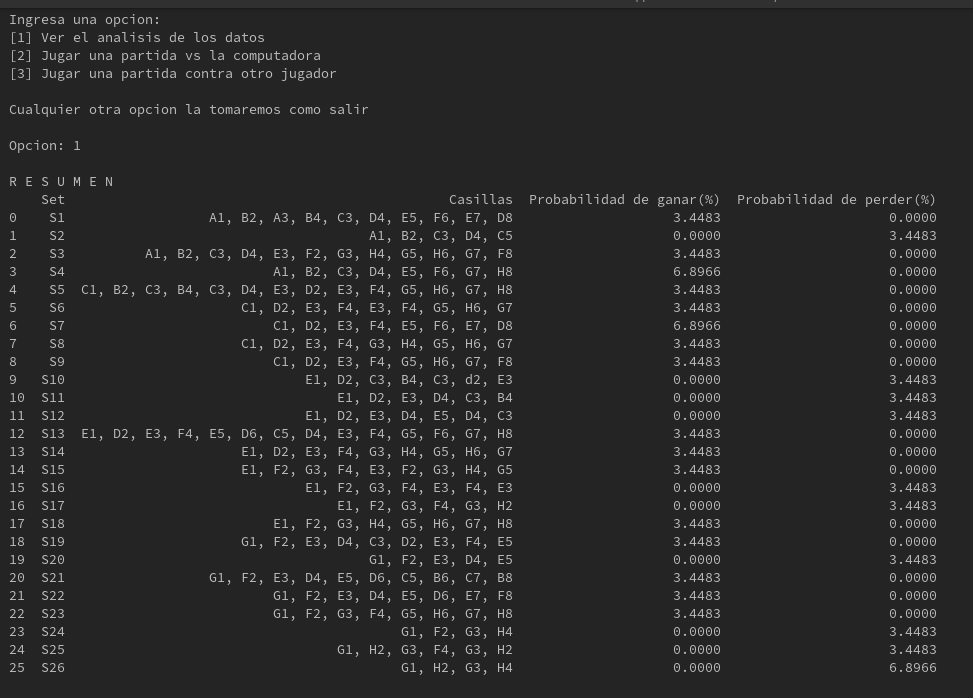
\includegraphics[scale=0.4]{Resultados1.png}
	\end{figure}
	\begin{figure}[H]
		\centering
		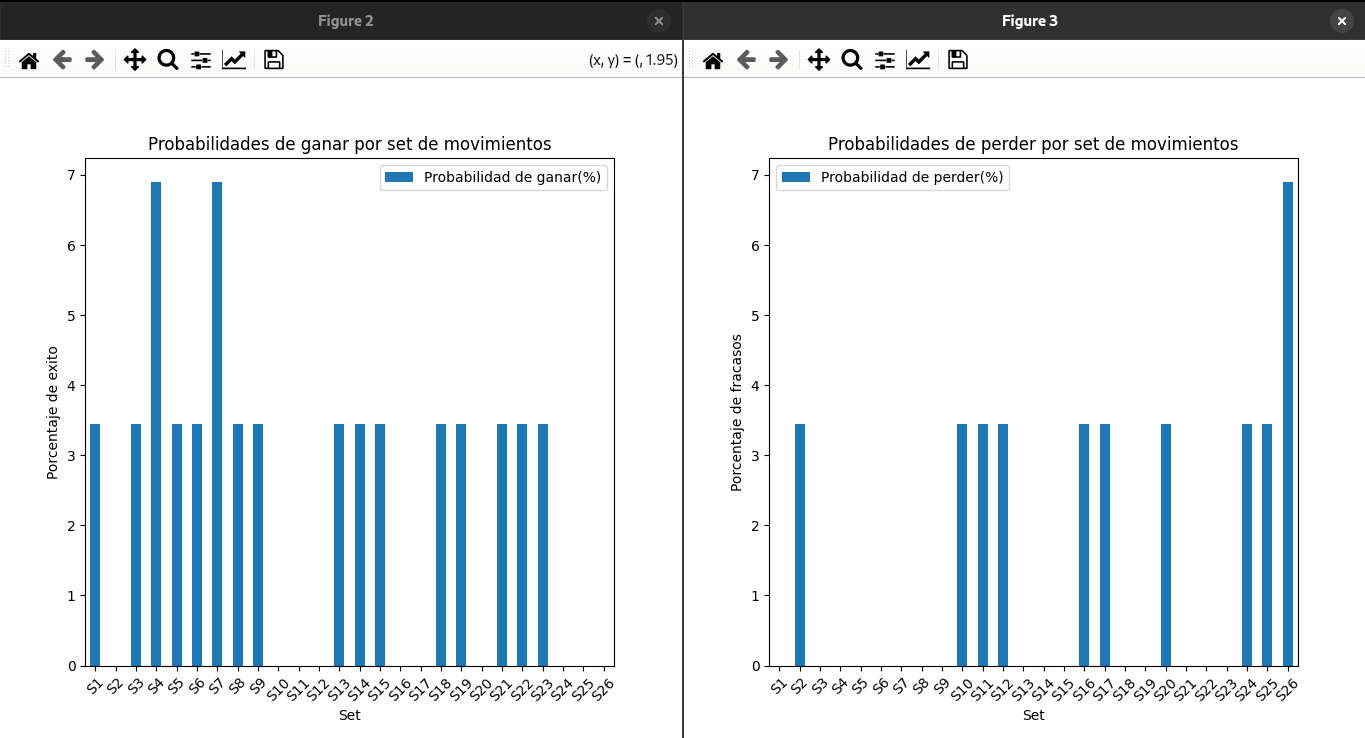
\includegraphics[scale=0.35]{Resultados2.png}
	\end{figure}
	
	
	\textbf{Uso como PyGame (Juego VS CPU Y PERDER): }
	\begin{figure}[H]
		\centering
		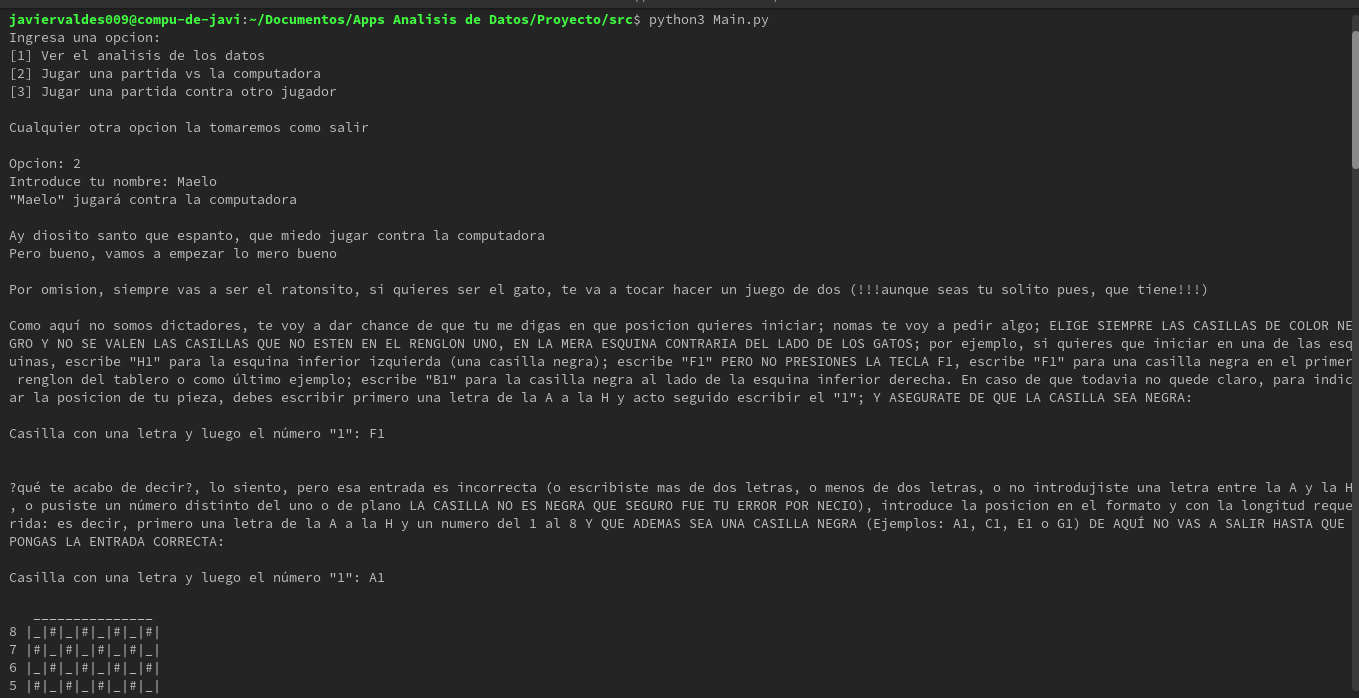
\includegraphics[scale=0.3]{Resultados3.png}
	\end{figure}
	\begin{figure}[H]
		\centering
		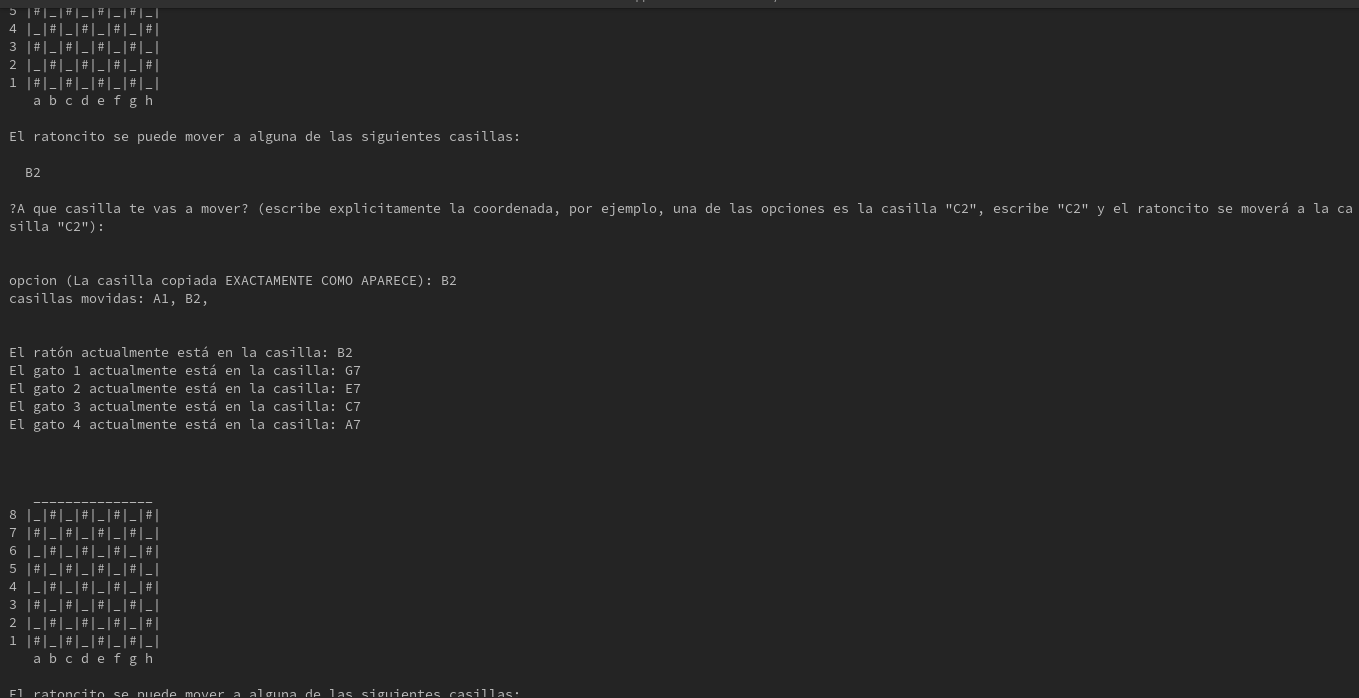
\includegraphics[scale=0.3]{Resultados4.png}
	\end{figure}
	\begin{figure}[H]
		\centering
		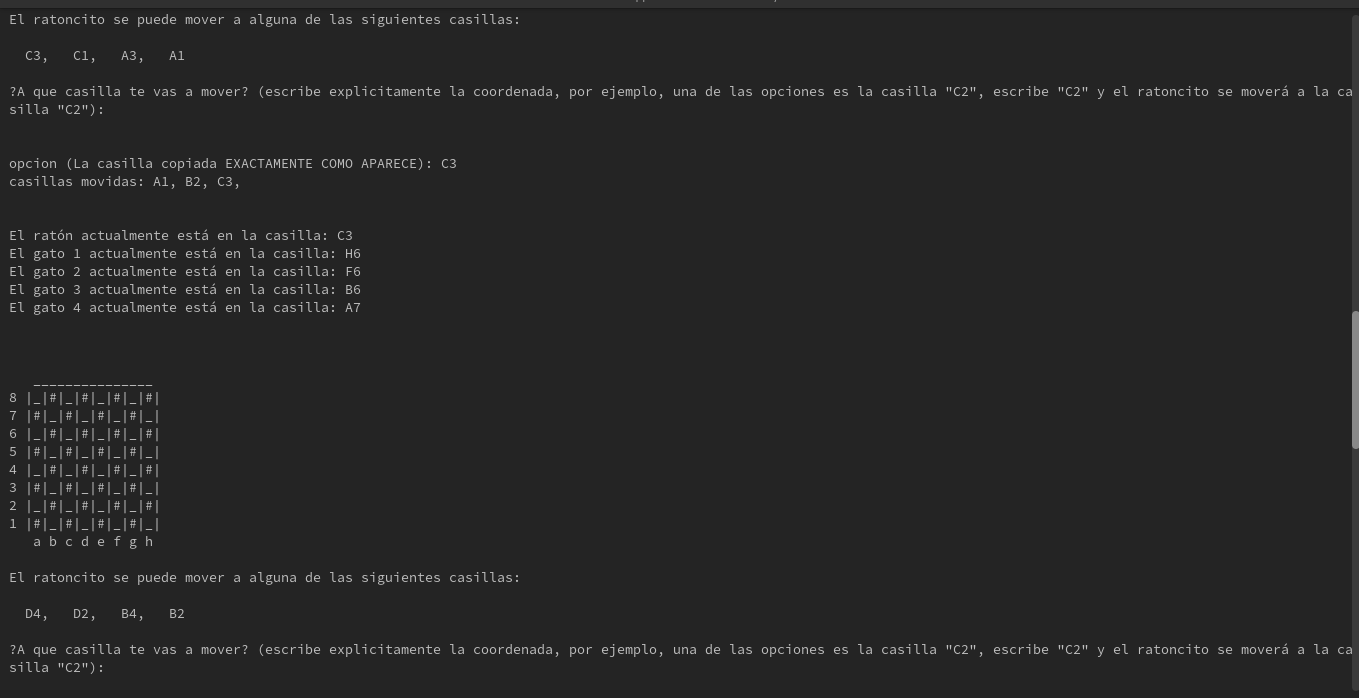
\includegraphics[scale=0.3]{Resultados5.png}
	\end{figure}
	\begin{figure}[H]
		\centering
		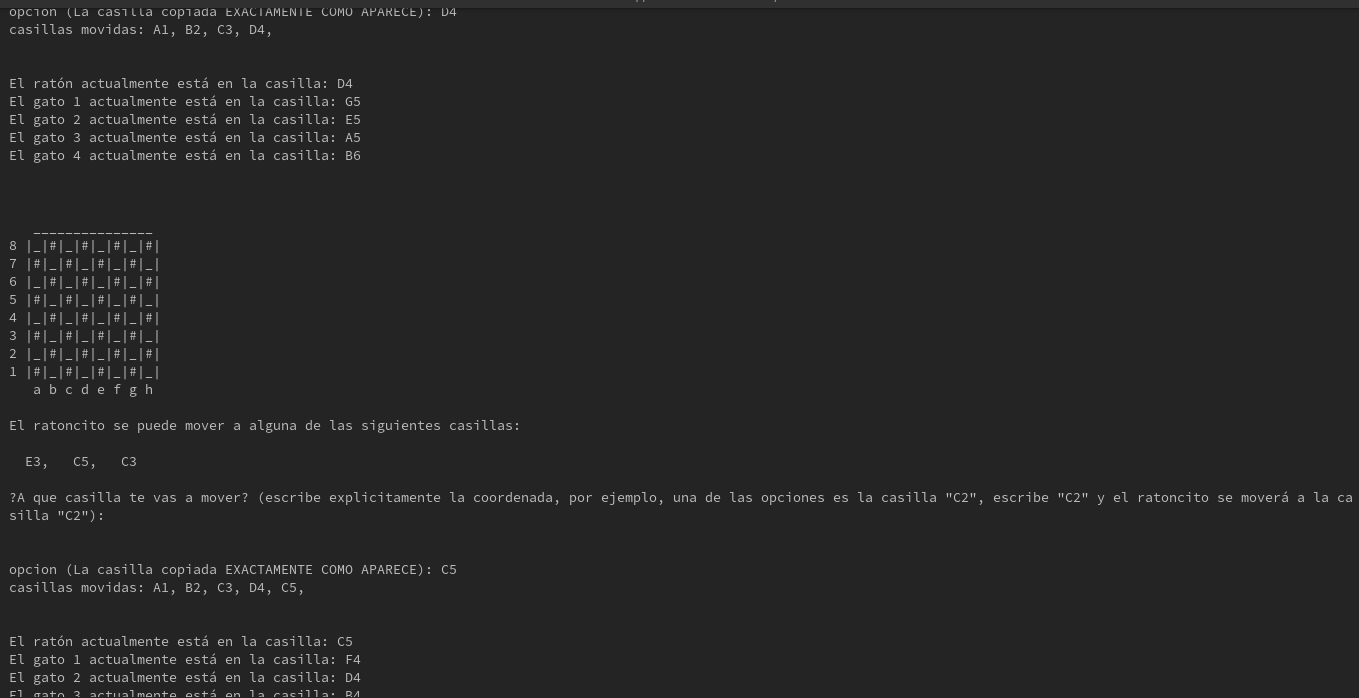
\includegraphics[scale=0.3]{Resultados6.png}
	\end{figure}
	\begin{figure}[H]
		\centering
		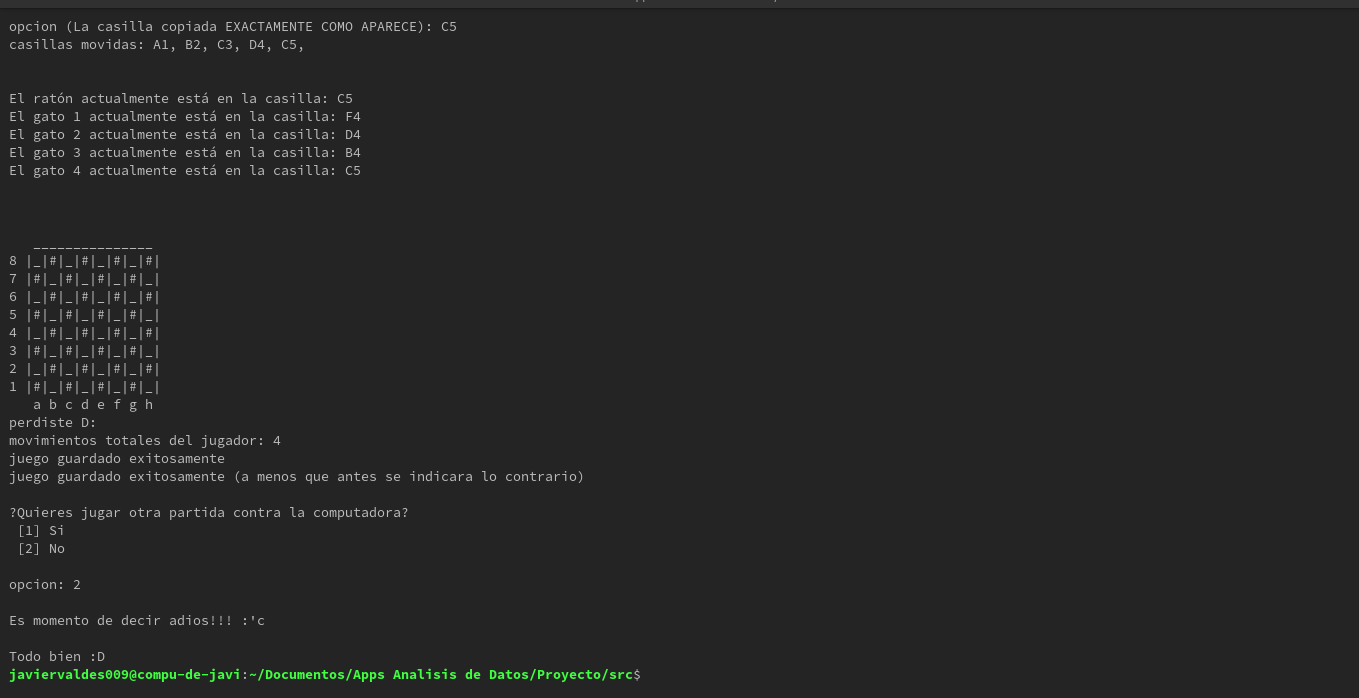
\includegraphics[scale=0.3]{Resultados7.png}
	\end{figure}
	
	
	\textbf{Uso como PyGame (Juego PVP): }
	\begin{figure}[H]
		\centering
		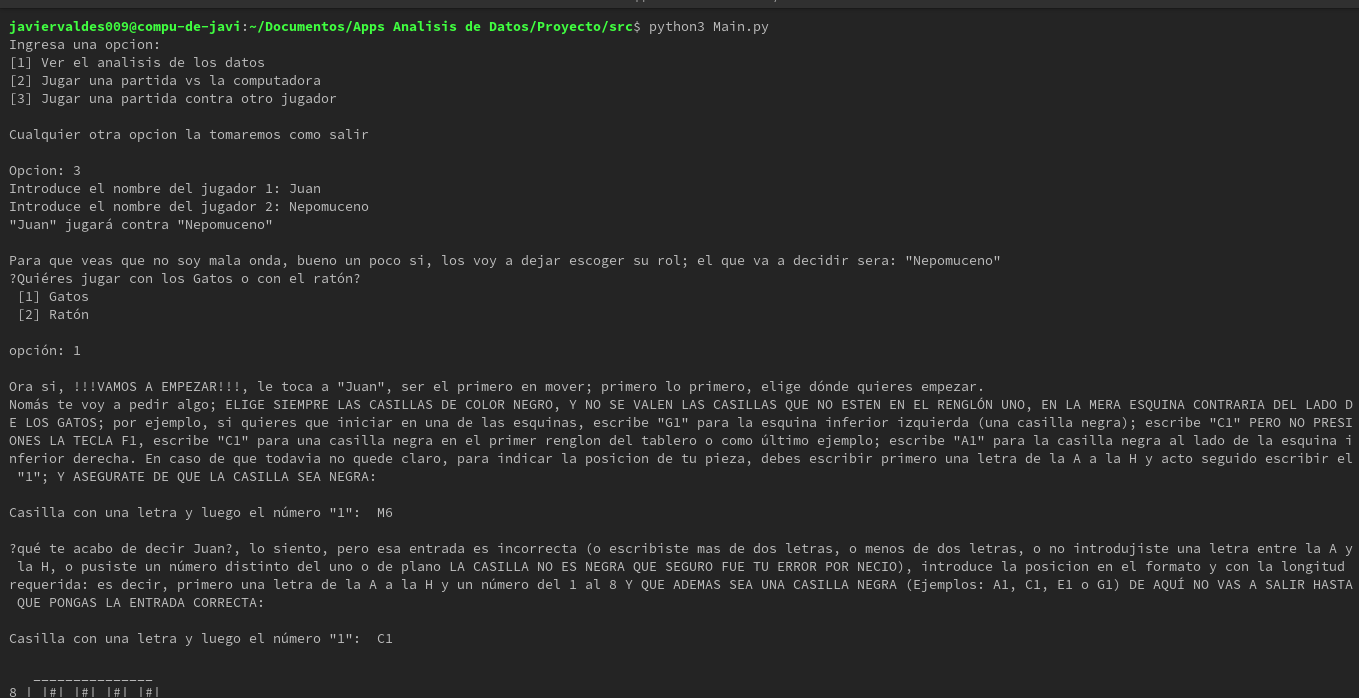
\includegraphics[scale=0.3]{Resultados8.png}
	\end{figure}
	\begin{figure}[H]
		\centering
		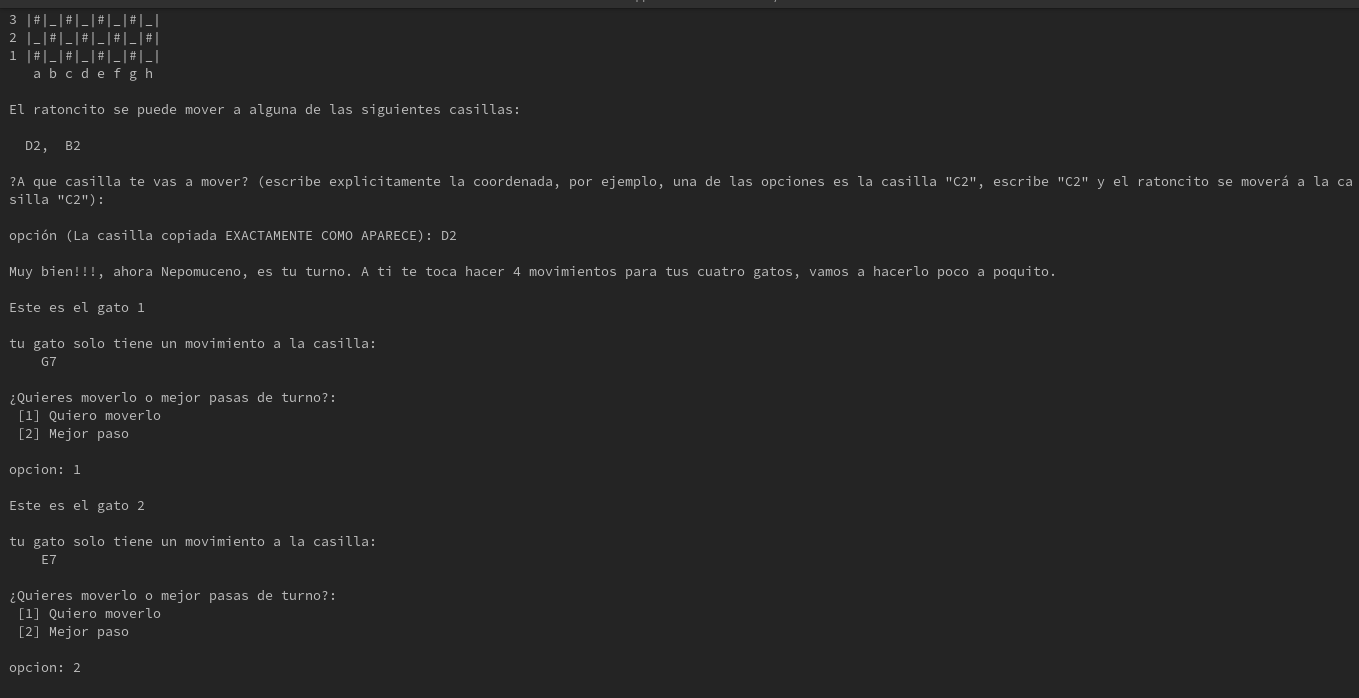
\includegraphics[scale=0.3]{Resultados9.png}
	\end{figure}
	\begin{figure}[H]
		\centering
		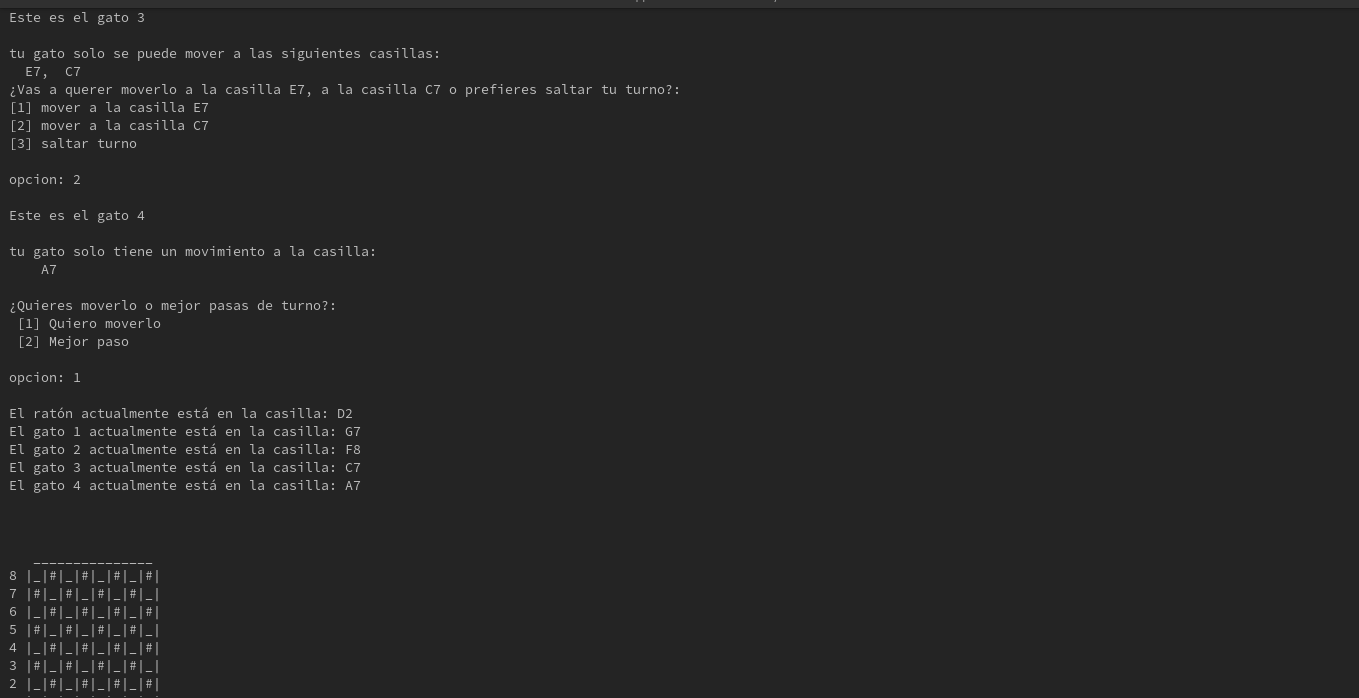
\includegraphics[scale=0.3]{Resultados10.png}
	\end{figure}
	\begin{figure}[H]
		\centering
		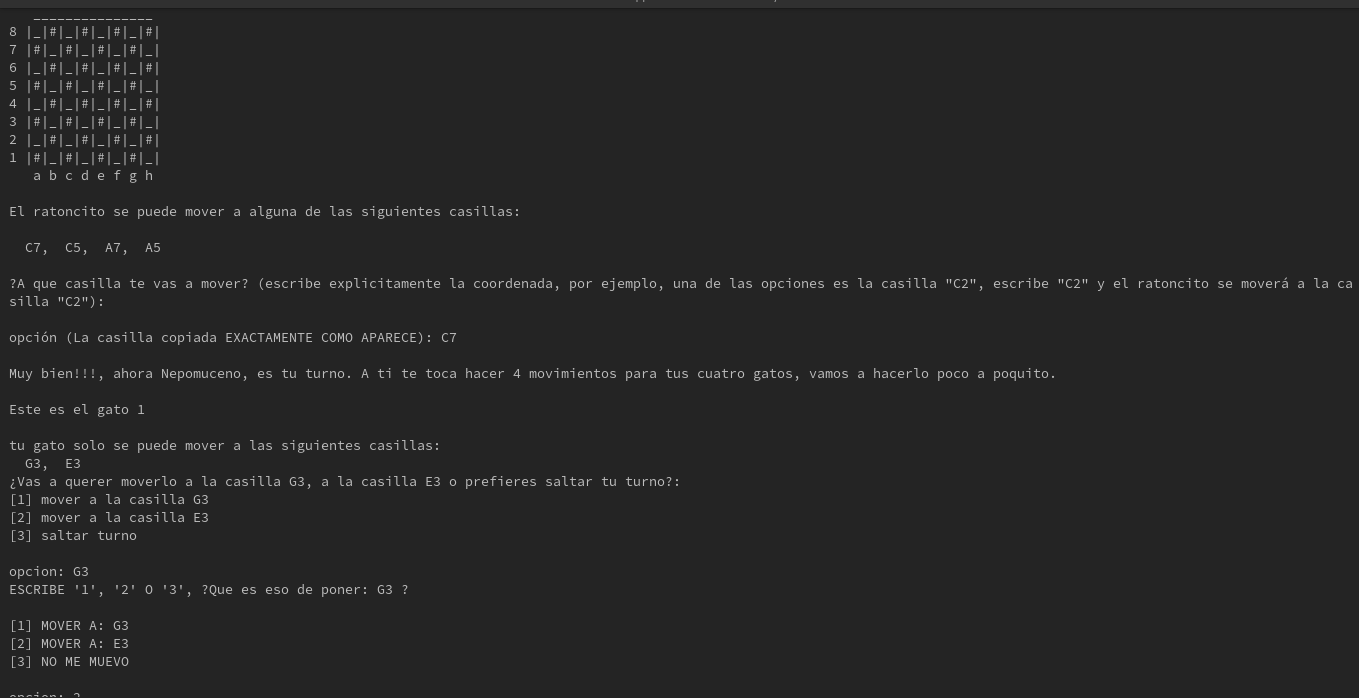
\includegraphics[scale=0.3]{Resultados11.png}
	\end{figure}
	\begin{figure}[H]
		\centering
		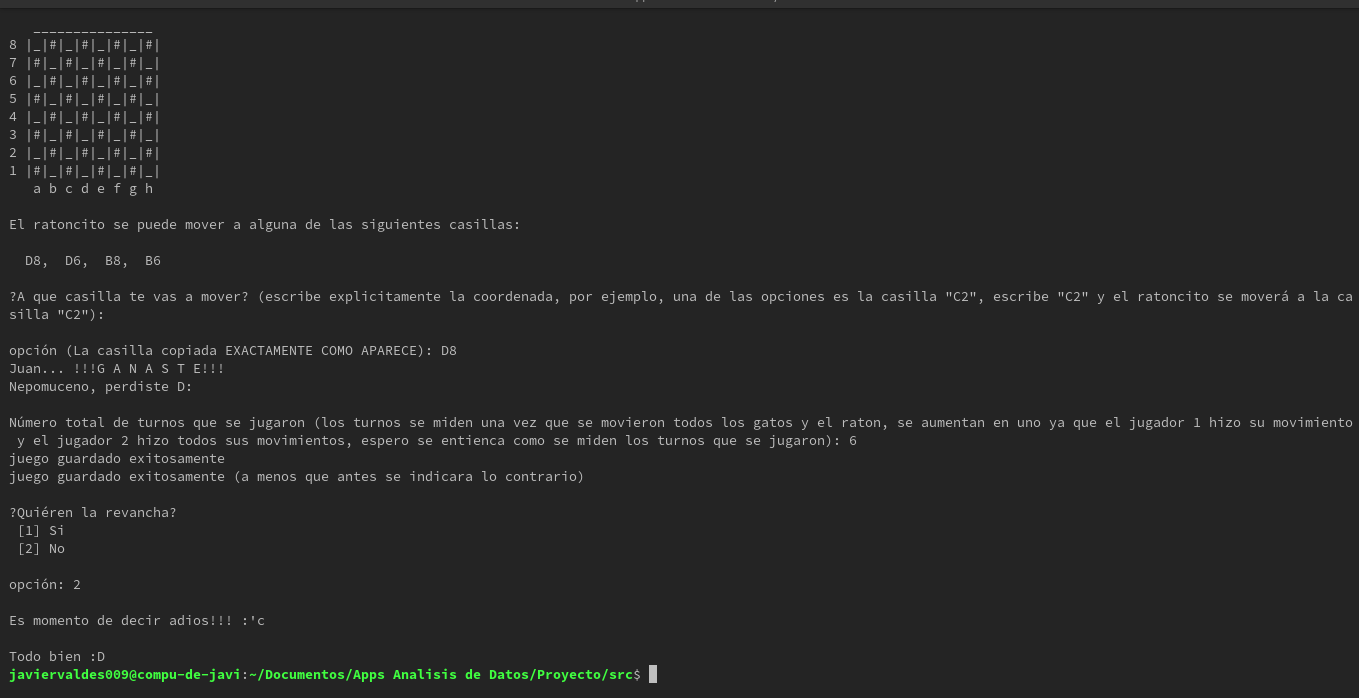
\includegraphics[scale=0.3]{Resultados12.png}
	\end{figure}
	
	
	
\end{document}
